\section{System Design}
\label{sec:fdsp-tpcelec-design}

%%%%%%%%%%%%%%%%%%%%%%%%%%%%%%%%%%%
\subsection{Grounding and Shielding}
\label{sec:fdsp-tpcelec-design-grounding}

%%%%%%%%%%%%%%%%%%%%%%%%%%%%%%%%%%%
\subsection{Distribution of Bias Voltages}
\label{sec:fdsp-tpcelec-design-bias}

%%%%%%%%%%%%%%%%%%%%%%%%%%%%%%%%%%%
\subsection{Front-End Motherboard}
\label{sec:fdsp-tpcelec-design-femb}

%%%%%%%%%%%%%%%%%%
\subsubsection{Overview}
\label{sec:fdsp-tpcelec-design-femb-overview}

Each \dword{apa} is instrumented with \num{20} %Front End Mother Boards (
\dwords{femb}.
The \dwords{femb} plug into the \dword{apa} CR boards, making the connections from the wires to the charge amplifier circuits as short as possible.
Each \dword{femb} receives signals from \num{40} $U$ wires, \num{40} $V$ wires, and \num{48} $X$ wires.
The baseline \dword{femb} design contains eight \num{16}-channel \dword{fe} (\dword{larasic}) \dwords{asic}, eight \num{16}-channel Cold \dword{adc} \dwords{asic}, and two \dword{coldata} control and communication \dwords{asic} (see Figure~\ref{fig:ce-scheme}).
The \dword{femb} also contains regulators that produce the voltages required by the \dwords{asic} and 
filter those voltages.
The \dword{larasic} inputs are protected by diodes and a series inductor.

\begin{dunefigure}
[The baseline \dword{ce} architecture.]
{fig:ce-scheme}
{The baseline \dword{ce} architecture. The basic unit is the \num{128}-channel \dword{femb}. Note that only one \dword{ce} flange is shown to simplify the illustration. Note that \dword{ssp} stands for \textit{SiPM Signal Processor} (see Chapter~\ref{ch:fdsp-pd}).}
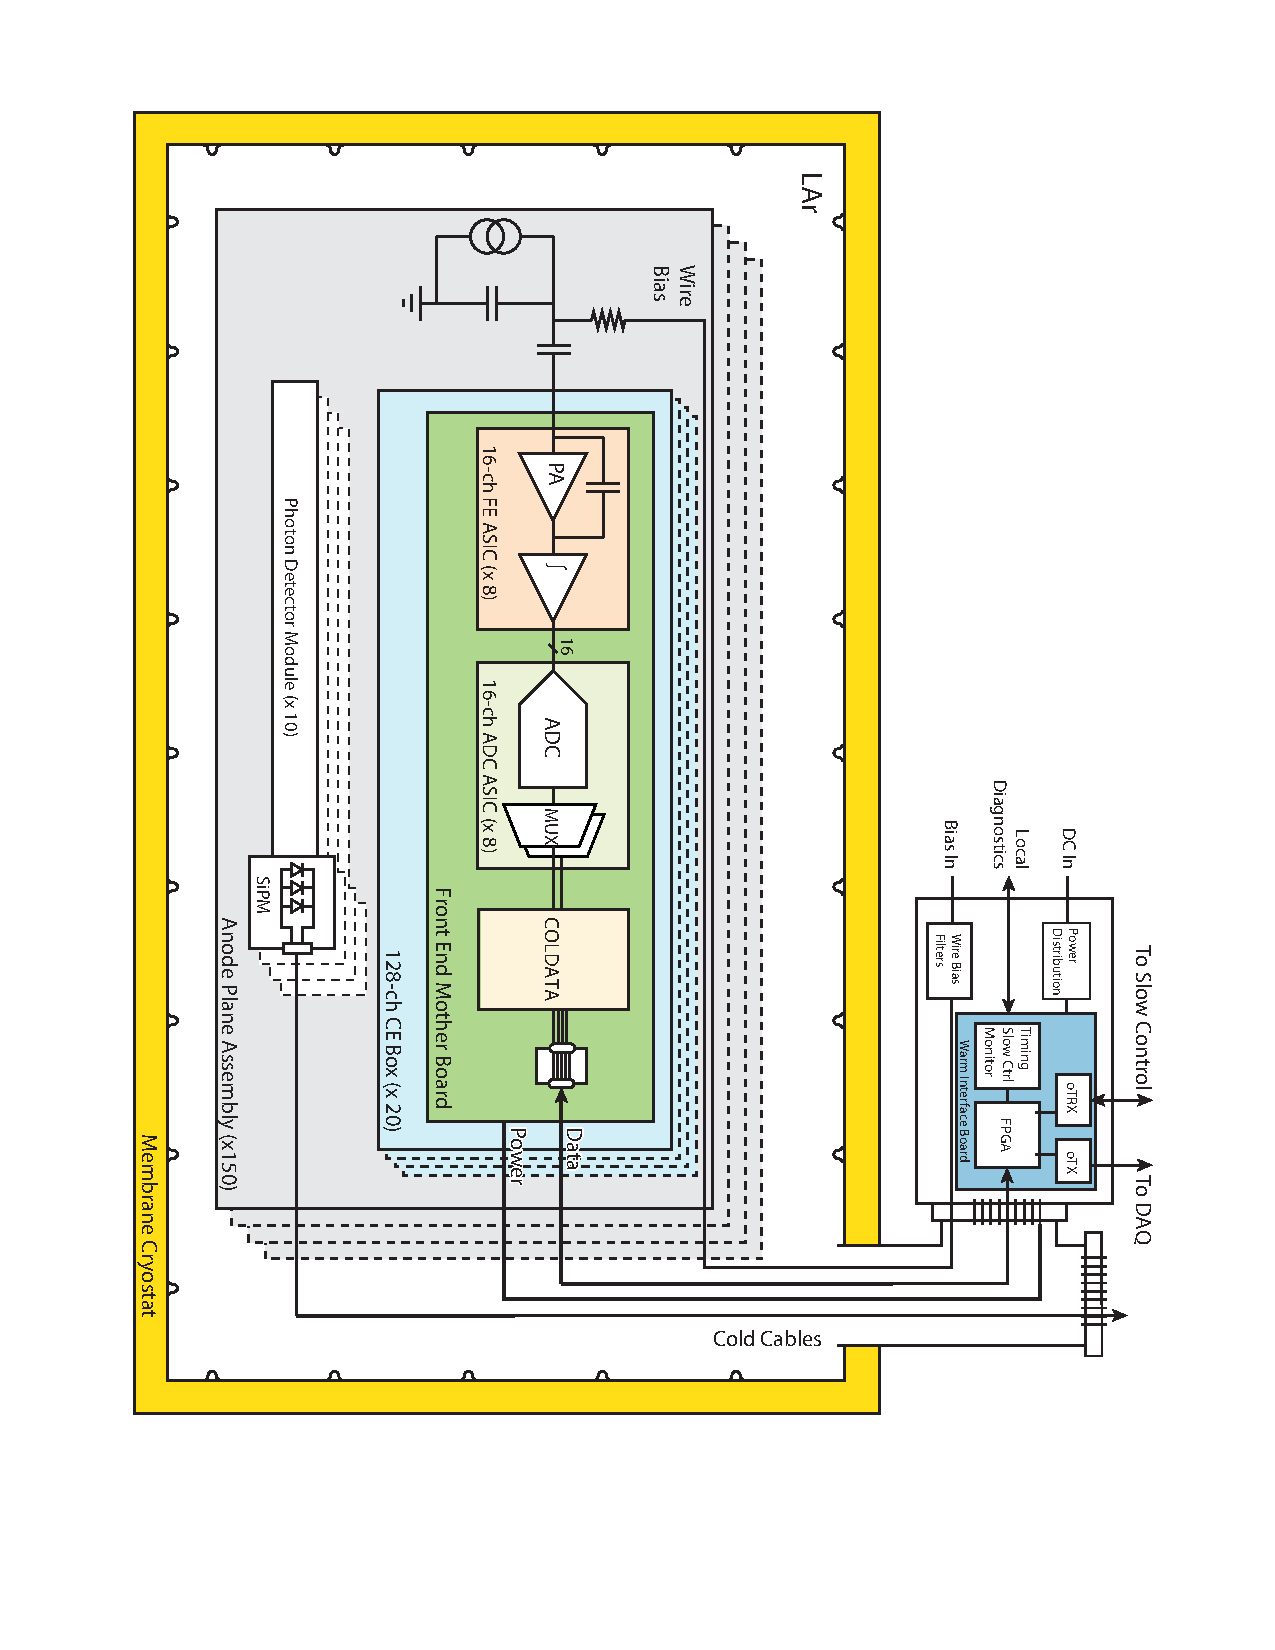
\includegraphics[width=0.9\linewidth,angle=90]{sp-tpcelec-schematic-v3.pdf}
\end{dunefigure}

The \dword{pdsp} version of the \dword{femb} (which uses a single \dword{fpga} on a mezzanine card instead of two \dword{coldata} \dwords{asic}) is shown in Figure~\ref{fig:femb}.

\begin{dunefigure}
[The complete \dword{femb} assembly as used in \dword{pdsp}.]
{fig:femb}
{The complete \dword{femb} assembly as used in the \dword{pdsp} detector. The cable shown is the high-speed data, clock, and control cable.}
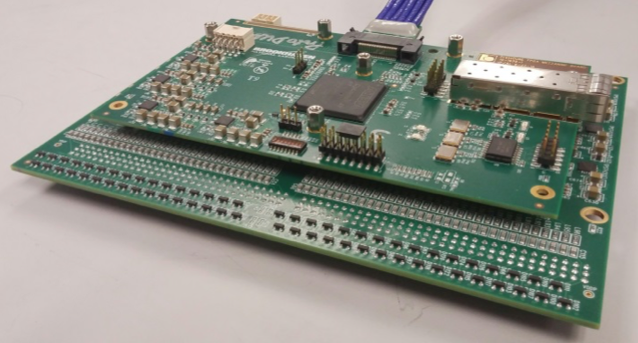
\includegraphics[width=0.6\linewidth]{sp-tpcelec-femb.png}
\end{dunefigure}

%%%%%%%%%%%%%%%%%%
\subsubsection{Front-End ASIC}
\label{sec:fdsp-tpcelec-design-femb-fe}

The analog front-end (FE) ASIC\cite{DeGeronimo:2011zz} receives current signals from the TPC sense wires and provides a means to amplify and shape the signals for downstream signal digitization.  The FE ASIC has 16 channels, and is implemented using the TSMC 180nm CMOS process. It integrates a band-gap reference (BGR) to generate all the internal bias voltages and currents. This guarantees a high stability of the operating point over a wide range of temperatures, including cryogenic temperatures. The channel schematic of the FE ASIC is shown in Figure~\ref{fig:feasic1}. 

\begin{dunefigure}
[FE ASIC channel schematic]
{fig:feasic1}
{Channel schematic of FE ASIC, which includes a dual-stage charge amplifier and a 5$^{th}$ order semi-Gaussian shaper with complex conjugate poles. Circuits in red circles are programmable to allow different gain and peaking time settings.}
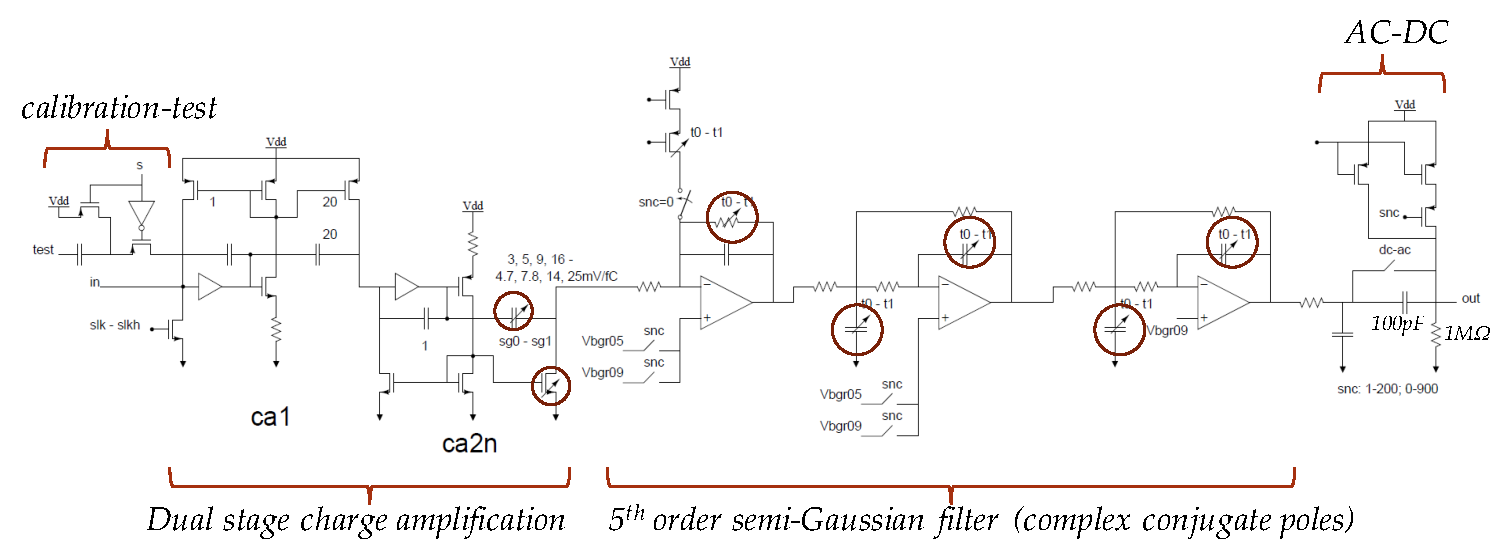
\includegraphics[width=0.99\linewidth]{sp-tpcelec-feasic-channelschematic.pdf}
\end{dunefigure}

Each FE ASIC channel has a dual-stage charge amplifier and a 5$^{th}$ order semi-Gaussian shaper as an anti-aliasing filter for the TPC signals. It has a programmable gain selectable from one of 4.7, 7.8, 14 or 25mV/fC (corresponding to full-scale charge of 300, 180, 100 and 55 fC), a programmable peaking time selectable from one of 0.5, 1, 2, and 3 $\mu$s, and a programmable baseline for operation with either the collection ($\sim$200mV) or the induction ($\sim$900mV) wires. Each channel has an option to enable the output monitor to probe the analog signal, and an option to enable a high-performance output driver that can be used to drive a long cable. 

Each FE ASIC channel has a built-in charge calibration capacitor which can be enabled or disabled through a dedicated register. The injection capacitance has been measured using a calibrated external capacitor. The measurements show that the calibration capacitance is extremely stable, changing from 184 fF at room temperature to 183 fF at 77 K. This result and the measured stability of the peaking time demonstrate the high stability of the passive components as a function of temperature. Channel-to-channel and chip-to-chip variation in the calibration capacitor are typically less than 1\%.

Shared among the 16 channels in the FE ASIC are the digital interface, programming registers, a temperature monitor and a bandgap reference monitor. It also has an option to enable AC coupling as mitigation of microphonics, a programmable bias current selectable from one of 0.1, 0.5, 1 or 5nA, and a programmable pulser generator with 6-bit DAC for calibration. 

The power dissipation of FE ASIC is about 5.5mW per channel at 1.8V supply voltage with output buffer disabled. The ASIC is packaged in a commercial, fully encapsulated plastic QFP 80 package. Figure~\ref{fig:feasic2} shows the response of FE ASIC for all gains and peaking times and both baselines. Note that the gain is independent of the peaking time; the same amount of charge produces the same peak voltage signal regardless of the peaking time.

\begin{dunefigure}
[FE ASIC response and layout]
{fig:feasic2}
{Response of FE ASIC for four gains, four peaking times, and both baseline values (left); layout of 16-channel FE ASIC version P3, where revisions with reference to version P2 are highlighted in yellow boxes (right).}
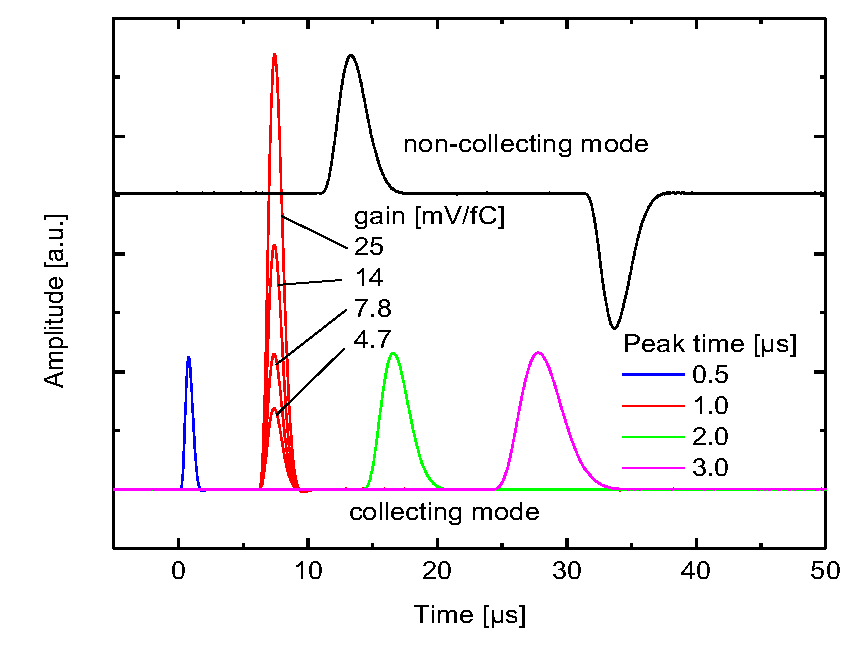
\includegraphics[width=0.48\linewidth]{sp-tpcelec-feasic-response.pdf}
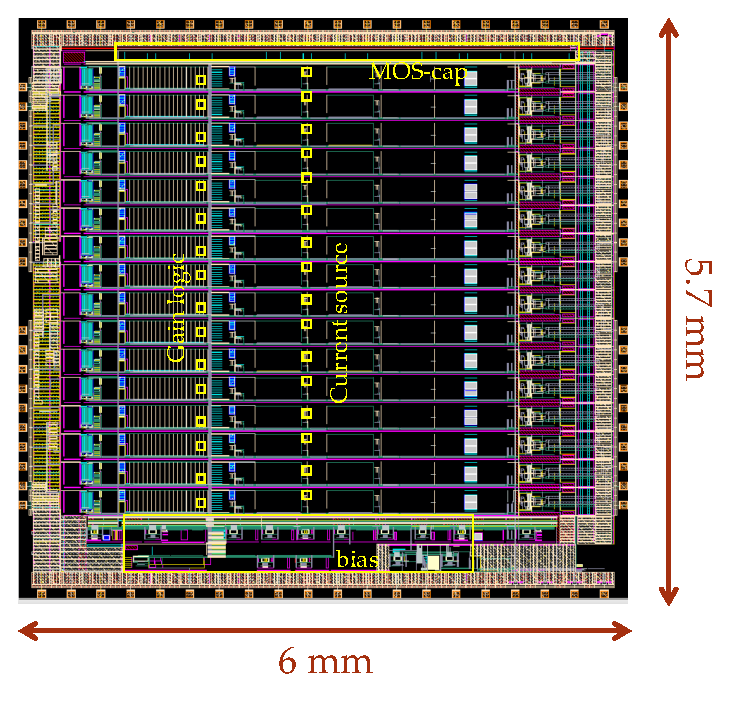
\includegraphics[width=0.48\linewidth]{sp-tpcelec-feasic-layout.pdf}
\end{dunefigure}

Prototype version P2 FE ASICs have been evaluated and characterized at room temperature and LN$_2$ (77 K) temperature. 960 P2 FE ASICs, total 15,360 channels, have been used to instrument six ProtoDUNE-SP APAs successfully. Due to exessive stress of package of FE ASIC in cryogenic temperature, FE channels have non-uniform baseline in collection mode, while the baseline DC voltage in induction mode is uniform. A new prototype version P3 has been fabricated in March 2018 to address this issue by making DC circuits for collection mode similar to the induction mode. At the same time, the default gain setting is changed to 14mV/fC. The layout of P3 FE ASIC is shown in \ref{fig:feasic2}, with modifications highlighted in yellow boxes. The P3 FE ASICs have been received and evaluated in September 2018, which shows both baseline in collection mode and default gain setting are working properly.

P3 FE ASIC will be further evaluated on FEMBs in various integration test stands for performance studies, including 40\% APA at BNL, ICEBERG TPC at Fermilab and APA7 at CERN. Test results of P3 FE ASIC will guide the development of next version P4 FE ASIC, which currently has a plan to implement single ended to differential (SE-DIFF) converter for interface to recently developed ADC ASIC. During the ProtoDUNE-SP operation, it was observed that the FE ASICs may enter into a saturation mode when large amount of charge ($>$ 50fC) is collected in the period of 10-50$\mu$s. This is being studied in the lab test stand, with the plan to address it in the P4 FE ASIC revision as well.

%%%%%%%%%%%%%%%%%%
\subsubsection{ADC ASIC}
\label{sec:fdsp-tpcelec-design-femb-adc}

%%%%%%%%%%%%%%%%%%
\subsubsection{COLDATA ASIC}
\label{sec:fdsp-tpcelec-design-femb-coldata}

%%%%%%%%%%%%%%%%%%
\subsubsection{Alternative Designs}
\label{sec:fdsp-tpcelec-design-femb-alt}

%%%%%%%%%
\subsubsection{CRYO}
\label{sec:fdsp-tpcelec-design-femb-alt-cryo}

%%%%%%%%%
\subsubsection{COTS (Commercial Off The Shelf)}
\label{sec:fdsp-tpcelec-design-femb-alt-cots}



%%%%%%%%%%%%%%%%%%
\subsubsection{Procedure and Timeline for ASIC Selection}
\label{sec:fdsp-tpcelec-design-femb-selection}

%%%%%%%%%%%%%%%%%%%%%%%%%%%%%%%%%%%
\subsection{Infrastructure Inside the Cryostat}
\label{sec:fdsp-tpcelec-design-infrastructure}

%%%%%%%%%%%%%%%%%%%%%%%%%%%%%%%%%%%
\subsection{Cold Electronics Feedthroughs}
\label{sec:fdsp-tpcelec-design-ft}

%%%%%%%%%%%%%%%%%%%%%%%%%%%%%%%%%%%
\subsection{Warm Interface Electronics}
\label{sec:fdsp-tpcelec-design-warm}

%%%%%%%%%%%%%%%%%%%%%%%%%%%%%%%%%%%
\subsection{Services on Top of the Cryostat}
\label{sec:fdsp-tpcelec-design-services}
